
We are going to discuss about two tools for cryptographic protocol verification: \href{https://prosecco.gforge.inria.fr/personal/bblanche/proverif/}{Proverif} and \href{https://tamarin-prover.github.io/}{Tamarin-Prover}. Tamarin-Prover will also be referred to as Tamarin for brevity.

First of all, let us consider the different types of approaches to security protocol analysis. The two categories of techniques are shown in \cref{fig:symbolic-computational-model} and we will proceed examining them.

\begin{figure}[t]
    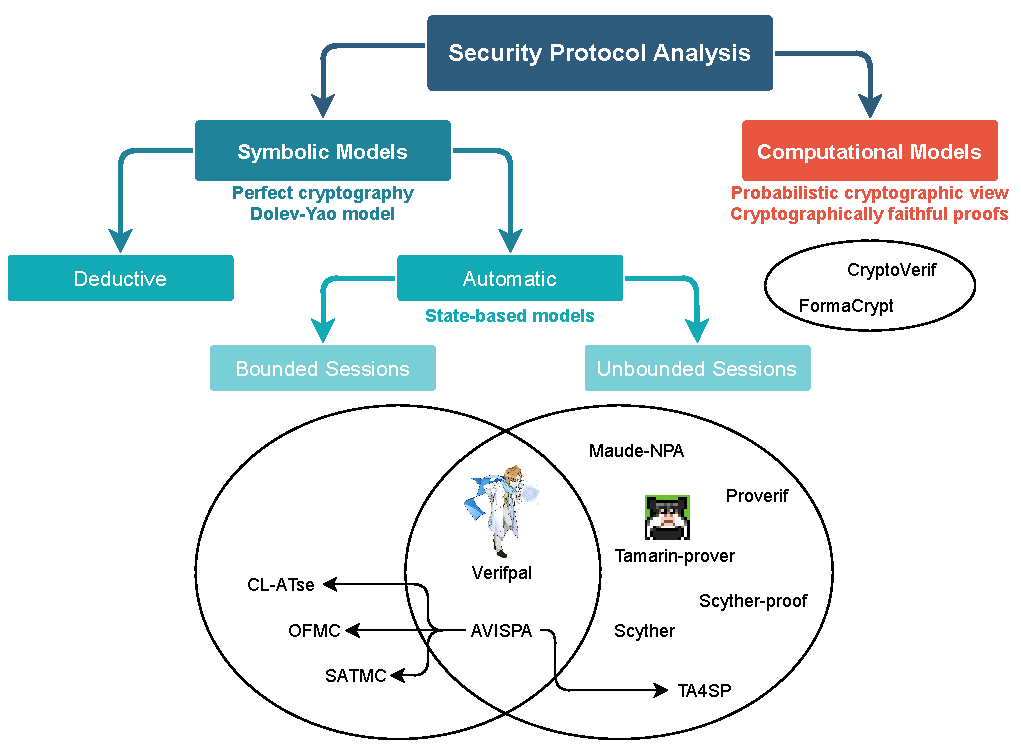
\includegraphics[scale=0.9]{symbolic-computational-model}
    \centering
    \caption{Symbolic and computational models}
    \label{fig:symbolic-computational-model}
\end{figure}

In the \textit{symbolic model} (often called Dolev-Yao model) \cite{Dolev-Yao}, the cryptographic primitives are considered as black-box and are represented using function symbols, the messages are terms and the adversary can only use defined primitives. An important aspect to note of this model is that it assumes \textbf{perfect cryptography}. As an example, consider the case in which there are two function symbols (\textbf{enc} and \textbf{dec}, used to encrypt and decrypt), a message \textit{m} and a key \textit{k} and the following equality is defined:

\begin{equation}
\mbox{dec}\left(\mbox{enc}\left(m, k\right), k\right) = m
\end{equation}

Following from the equation $-$ and considering the perfect cryptography assumption $-$ it is possible to decrypt $\mbox{enc}\left(m, k\right)$ if and only if \textit{k} is known \cite{SymbolicComputationalBlanchet}.


In the \textit{computational model} the messages are bitstrings, the cryptographic primitives are functions from bitstrings to bitstrings and the attacker is modeled as a probabilistic Turing machine.
A security property in this model is considered to hold when the probability that it does \textit{not} hold is negligible. For instance, the previously discussed shared-key encryption can be modeled using the same equalities, but the security of encryption is expressed by stating that the attacker has an insignificant probability of breaking the primitive (e.g. decrypting the message without having the key). Security proofs using this model are usually stronger, however this comes to the cost of long, difficult, tedious and highly error prone proofs (as stated by INRIA researchers \cite{ComputationalAnalysisCryptoSystemsINRIA}). Finally, as pointed to by Blanchet \cite{SymbolicComputationalBlanchet}, the computational model is indeed just a \textit{model} and ignores many aspects of reality and potential attacks, e.g. faulty attacks like the one affecting processors computing RSA signatures \cite{RSAFaultAttack}. 

Both Proverif and Tamarin employ a symbolic model. This makes it possible to automate proofs when given a set of primitives, a protocol model and a set of security properties. Note that termination is still not always guaranteed\footnote{It actually depends on the tool. Proverif proofs always terminate, but they might terminate with an inconclusive result, while Tamarin may simply not terminate without ever giving a result. More details about this problem will be discussed later.}. % TODO: discuss non termination issues!!

\section{Difficulties in the security protocol analysis in the symbolic model}
There are two main problems that affect most tools for security protocol analysis: \textbf{infinite state space} and \textbf{undecidability}.

At an high level, to verify a protocol in the symbolic model, one computes the set of terms that the adversary knows. If a certain term does not belong to this set, then the term is considered secret \cite{SymbolicVerificationBlanchet}. The difficulty is that the set of terms is infinite. Specifically, we have three sources of infinity when analyzing a protocol:
\begin{description}
    \item[\textbf{Messages}] - the adversary can produce messages of any arbitrary size;
    \item[\textbf{Sessions}] - as many attacks are possible only when multiple sessions are executed in parallel, symbolic models often use an unbounded number of sessions;
    \item[\textbf{Nonces}] - if we have an unbounded number of session, then we also must have an unbounded number of nonces to use in those sessions.
\end{description}

There have been various way of tackling this problem:
\begin{itemize}
    \item{It is possible to decide to bound every source of infinity. In this case the state space is actually finite. This method was used, for example, by Lowe \cite{LoweNeedhamSchroederPK} and SATMC \cite{SATMC};}

    \item{We can bound the number of executions of the protocol. This still leads to an infinite state space, but \cite{SymbolicModelNPCompleteInsecurity} have shown that insecurity is NP-complete;}
    
    \item{If we do not force any bound, the problem becomes undecidable \cite{SymbolicModelUndecidability1} \cite{SymbolicModelUndecidability2}. As pointed out by \cite{SymbolicVerificationBlanchet}, no automatic tool that always terminates and solves the problem can exist. For a given protocol, it is not possible to determine if the proof will, eventually, end. \Cref{fig:undecidability} shows the boundary of decidability. As evidenced by the diagram, the problem is decidable if and only if we bound at least two sources of infinity out of three.

    Of course, there are several approaches to confront this problem:

    \begin{itemize}
        \item{Rely on help from the user. This is the approach chosen by Tamarin \cite{TamarinFoundations}, which allows for semi-automatic proofs (possible messages are ranked by the system, but the user can chose which to solve first);}
        \item{Another possibility is to have tools that may return an inconclusive result $-$ yet are supposed to work correctly in most cases;}
        \item{The last approach is to allow non-termintion.}
    \end{itemize}
    }
\end{itemize}


\begin{figure}[t]
    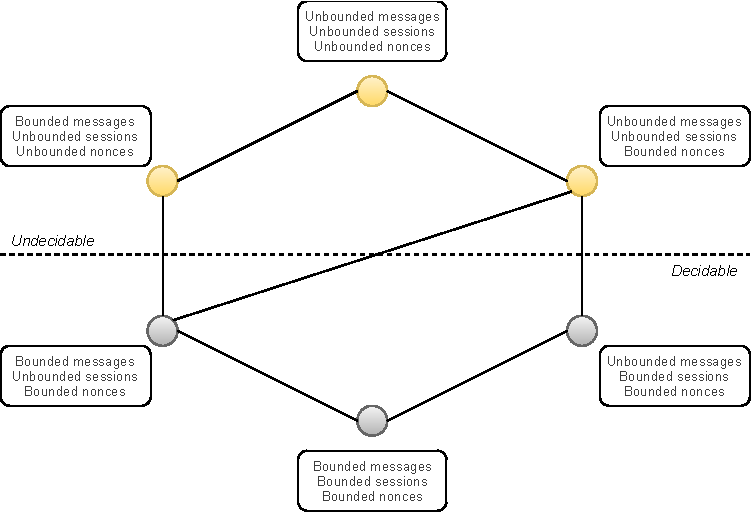
\includegraphics{undecidability}
    \centering
    \caption{Decidability of termination.\\Heavily inspired by a representation by Nicola Vitacolonna.}
    \label{fig:undecidability}
\end{figure}

\section{Proverif}
% TODO

\section{Tamarin}
In this section we will see an overview of Tamarin foundations and internal reasoning.
For a more in-depth description and further information, see the Tamarin foundations paper \cite{TamarinFoundations} or the extended foundations paper \cite{TamarinFoundationsExtended}.

\subsection{High level view}
First of all, let us examine an high level picture of Tamarin.

The security property model of Tamarin is based on labelled multiset rewriting rules to specify protocols and adversary capabilities, a guarded fragment\footnote{Only a few examples of formulas respecting the guarded fragment of first order logic used by Tamarin will be given in the next subsections. See \cite{FragmentFirstOrderLogicPaper} for a rigorous definition from a mathematical point of view.} of first order logic to specify security properties\footnote{Security properties in Tamarin will also be referred to as \textit{lemmas}.} and functions and equational theories to model the algebraic properties of cryptographic protocols \cite{TamarinFoundations}. % TODO: show a few examples of first order logic formulas respecting the guarded fragment!!

Given the rewriting rules, security properties and equational theories, Tamarin uses a novel constraint-solving algorithm which tries to validate or falsify lemmas.

In other words, Tamarin allows to specify a labelled transition system that induces a set of traces and offers verification of such traces using a guarded fragment of first-order logic to specify ``good" traces. Tamarin then tries to prove the negation of the specified ``good" traces.

Tamarin also offers builtin equational theories \cite{TamarinProverManual}. A brief overview will be given in \cref{sub:Builtin-equational-theories}.

\subsection{Terminology}
As reported earlier, multiset rewriting rules are used to specify adversary capabilities and protocols. More precisely, a \textit{set} of \textit{labelled} multiset rewriting rules are used.

The ingredients of this multiset rewriting system are the following: 

\begin{description}[style=nextline]
    \item[Terms] which can be essentially thought of as messages. Terms can be of three different sorts. The more general sort is the \textit{msg} sort, which has two incomparable subsorts \textit{fresh} and \textit{pub} for fresh and public names, respectively;
    \item[Facts] which model information in the protocol. Facts have an arity, can be linear or persistent and are composed by terms. Linear facts model resources that can be consumed once, while persistent facts can be consumed an arbitrary number of times (and are prefixed by an exclamation mark). By convention, facts always start with a capital letter;
    \item[Special facts] Four facts are reserved and are used to model the freshness of a message $t$ ($\mbox{\textbf{Fr}}\left(t\right)$), a message $t$ coming from the public channel ($\mbox{\textbf{In}}\left(t\right)$), a message $t$ to be output to the public channel ($\mbox{\textbf{Out}}\left(t\right)$) and knowledge of a certain message $t$ from the attacker ($\mbox{\textbf{K}}\left(t\right)$);
    \item[State of the system] The state of the system is represented using a \textit{multiset} of facts;
    \item[Transition rules] A multiset of transition rules defines the possible transitions from one state to another one. Transitions are denoted with the following syntax
    \begin{equation}
        L \msrewrite{A} R
    \end{equation}
    where $L, A$ and $R$ are multisets of facts, respectively called \textbf{premises}, \textbf{actions} and \textbf{conclusions}.
    \item[Trace] A trace is a sequence $\left<A_1, \dots, A_n\right>$ of sets of ground facts denoting the sequence of actions that happened during a protocol's execution.
\end{description}


\subsection{Transition rules}
\label{sub:Transition-rules}
Let us examine an informal description of transitions.

\begin{itemize}
    \item{Let $S$ be the current state of the system}
    \item{Let $\msrnolabel{L}{R}$ be a transition rule. Note that this is a \textit{multiset rewriting rule} without a \textit{label};}
    \item{Let $\msrnolabel{l}{r}$ be a ground instance of the rule (i.e. no variables are present in the multisets);}
    \item{If we apply $\msrnolabel{l}{r}$ (assuming $l \msrsubseteq S$) to our state $S$ we reach a new state, defined by the following equation:
    \begin{equation}
        S' = S \msrsetminus l \msrcup r
    \end{equation}
    We use $\msrsetminus$, $\msrcup$ and $\msrsubseteq$ to define difference, union and subset over multisets, respectively. We can also consider the difference between linear and persistent facts and define $\lin{l}$ ($\pers{l}$) as linear facts (persistent facts) in $l$. Assuming that $\lin{l} \msrsubseteq S$ and $\pers{l} \msrsubseteq S$, then the equation becomes the following:
    \begin{equation}
        S' = S \msrsetminus \lin{l} \msrcup r
    \end{equation}
    It should be fairly clear from the equation why persistent facts can be consumed any number of times: they are never removed from the state of the system. This can be useful in scenarios in which we want to model persistent knowledge (e.g. the establishment of an encryption key $k$ may be expressed by a persistent fact $\fact{Key}{k}$).
    }
    \item{When we use labelled multiset rewriting rules, such as $\msr{l}{a}{r}$, we also add facts from $a$ to the \textit{trace} of the execution.}
\end{itemize}

Some multiset rewriting rules are always defined by Tamarin:

\begin{equation}
\begin{gathered}
    \msr{!KU\left(x\right)}{K\left(x\right)}{In\left(x\right)}\\
    \msrnolabel{Out\left(x\right)}{!KD(x)}
\end{gathered}
\end{equation}


\subsection{Builtin equational theories}
\label{sub:Builtin-equational-theories}
A brief list of Tamarin built-ins is given below:\footnote{Only the builtin theories considered relevant and those used in the analysis will be described here. The full list is available in the Tamarin manual. \cite{TamarinProverManual}}

\begin{description}[style=nextline]
    \item[hashing] defines a perfect hash function \textbf{h/1}\footnote{The writing \textbf{f/x} indicates that the function \textbf{f} has arity \textbf{x}.};
    \item[asymmetric-encryption] models a public key encryption scheme. It defines the following symbols:
    
    \begin{itemize}
        \item{\textbf{aenc/2}, used to model the encryption of a message with a public key}
        \item{\textbf{adec/2}, used to model the decryption of an encrypted message with a private key}
        \item{\textbf{pk/1}, used to derive a public key from a private key}
    \end{itemize}

    Functions are related by the equation \textbf{adec(aenc(msg, pk(sk)), sk) = msg};

    \item[diffie-hellman] models Diffie-Hellman groups. It defines the following symbols:
    
    \begin{itemize}
        \item{\textbf{inv/1}, models the inverse of an element}
        \item{\textbf{1/0}, models the neutral element}
        \item{\textbf{\textasciicircum} and \textbf{*} symbols, models exponentiation and multiplication respectively}
    \end{itemize}

    The equational theory for this builtin is actually quite complex. For the sake of completeness, these are the related equations:
    \begin{itemize}
        \item{(x \textasciicircum y) \textasciicircum z = x \textasciicircum (y * z)}
        \item{x \textasciicircum 1 = x}
        \item{x * y = y * x}
        \item{(x * y) * z = x * (y * z)}
        \item{x * 1 = x}
        \item{x * inv(x) = 1}
    \end{itemize}
    % TODO: parla ancora un po' di quanto sia figo Tamarin che ha DH builtin!
\end{description}

\section{Comparison of Proverif and Tamarin}